\documentclass[a4paper,12pt]{article}
\usepackage{a4wide}
\usepackage{tikz}
\usetikzlibrary{calc}
\usepackage{hyperref}

\begin{document}
\pagestyle{empty}
\setlength{\parindent}{0em}
\section*{Arithmetic}

Your task is to program the behavior of an entity called "arithmetic". This entity is declared in the attached file "arithmetic.vhdl" and has the following properties:
\begin{itemize}
\item Inputs:  I1, I2 with type std\_logic\_vector
\item Outputs: O with type std\_logic\_vector , V with type std\_logic, C with type std\_logic, VALID with type std\_logic
\end{itemize}
\begin{center}
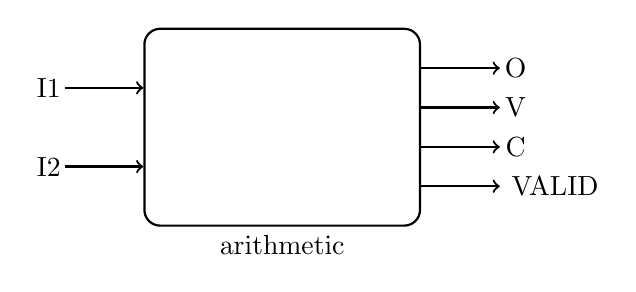
\begin{tikzpicture}
\draw node [draw,rectangle, minimum height=25mm, minimum width=35mm,rounded corners=2mm,thick](entity){};
\draw[->,thick] ($ (entity.west)-(10mm,5mm)$) -- ($ (entity.west) - (0mm,5mm)$);
\draw node at ($ (entity.west)-(12mm,5mm)$){I2};
\draw[->,thick] ($ (entity.west)-(10mm,-5mm)$) -- ($ (entity.west) - (0mm,-5mm)$);
\draw node at ($ (entity.west)-(12mm,-5mm)$){I1};

\draw[->,thick] ($ (entity.east) + (0mm,7.5mm)$) -- ($ (entity.east) + (10mm,7.5mm)$);
\draw node at ($ (entity.east) + (12mm,7.5mm)$){O};
\draw[->,thick] ($ (entity.east) + (0mm,2.5mm)$) -- ($ (entity.east) + (10mm,2.5mm)$);
\draw node at ($ (entity.east) + (12mm,2.5mm)$){V};
\draw[->,thick] ($ (entity.east) + (0mm,-2.5mm)$) -- ($ (entity.east) + (10mm,-2.5mm)$);
\draw node at ($ (entity.east) + (12mm,-2.5mm)$){C};
\draw[->,thick] ($ (entity.east) + (0mm,-7.5mm)$) -- ($ (entity.east) + (10mm,-7.5mm)$);
\draw node at ($ (entity.east) + (17mm,-7.5mm)$){VALID};


\draw node at ($ (entity) - (0,15mm)$){arithmetic};

\end{tikzpicture}
\end{center}

Do not change the file "arithmetic.vhdl".
\\

The entity shall implement the following arithmetic functionality:
\begin{itemize}
\item {{OPERATION_NAME}} I1 {{OPERATION_SIGN}} I2
\item Input operand 1 (I1): {{I1_WIDTH}} bit, {{OPERAND_STYLE}}
\item Input operand 2 (I2): {{I2_WIDTH}} bit, {{OPERAND_STYLE}}
\item Output (O): {{O_WIDTH}} bit, {{OPERAND_STYLE}}
\item Overflow (V) and Carry flag (C) set accordingly
\item Valid flag (VALID): indicates if the computed solution is valid or not
\end{itemize}

This behavior has to be programmed in the attached file "arithmetic\_beh.vhdl".


\textbf{Note:} The ALU has to be implemented using the width of {{O_WIDTH}} bit. Sign extension
of operands might be needed.


\rule{16cm}{0.4pt}\par
\subsection*{Review: Carry and Overflow Flag}

\textbf{Carry Flag}\\
The rules for turning on the carry flag in binary math are two:
\begin{enumerate}
\item The carry flag is set if the addition of two numbers causes a carry
   out of the most significant (leftmost) bits added.

   e.g. 1111 + 0001 = 0000 (carry flag is '1')

\item The carry (borrow) flag is also set if the subtraction of two numbers
   requires a borrow into the most significant (leftmost) bits subtracted.

   e.g. 0000 - 0001 = 1111 (carry flag is '1')

Otherwise, the carry flag is turned off ('0').
\begin{itemize}
\item e.g. 0111 + 0001 = 1000 (carry flag is '0')
\item e.g. 1000 - 0001 = 0111 (carry flag is '0')
\end{itemize}

%CHANGED: omit 1s complement
%In ones' complement the carry flag is set before a possible end around operation.

In unsigned arithmetic, watch the carry flag to detect errors.
In signed arithmetic, the carry flag tells you nothing interesting.

\end{enumerate}

\textbf{Overflow Flag}\\
The rules for turning on the overflow flag in binary math are two:
\begin{enumerate}
\item If the sum of two numbers with the sign bits off yields a result number
   with the sign bit on, the "overflow" flag is turned on.

   e.g. 0100 + 0100 = 1000 (overflow flag is '1')

\item If the sum of two numbers with the sign bits on yields a result number
   with the sign bit off, the "overflow" flag is turned on.

   e.g 1000 + 1000 = 0000 (overflow flag is '1')
\end{enumerate}

Otherwise, the overflow flag is turned off.
\begin{itemize}
\item e.g. 0100 + 0001 = 0101 (overflow flag is '0')
\item e.g. 0110 + 1001 = 1111 (overflow flag is '0')
\item e.g. 1000 + 0001 = 1001 (overflow flag is '0')
\item e.g. 1100 + 1100 = 1000 (overflow flag is '0')
\end{itemize}

%CHANGED: omit 1s complement
%In ones' complement the overflow flag is set after a possible end around operation.

If you are doing complement (signed) arithmetic, overflow flag on
means the answer is wrong - you added two positive numbers and got a
negative, or you added two negative numbers and got a positive. If you are doing unsigned arithmetic, 
the overflow flag does not give relevant information.

\vspace{0.5cm}
\textit{Source: }\url{http://teaching.idallen.com/dat2343/10f/notes/040_overflow.txt}
\\
\rule{16cm}{0.4pt}

\vspace{0.3cm}

Tip: Use the "ieee.numeric\_std" package to implement the arithmetic operation.
\\

To turn in your solution write an email to {{SUBMISSIONEMAIL}} with Subject "Result Task {{TASKNR}}" and attach your file "arithmetic\_beh.vhdl".

\vspace{0.7cm}
Good Luck and May the Force be with you.

\end{document}
